\section{Resultados Experimentais}

\subsection{Desempenho de Predição}
A Tabela~\ref{tab:pred_perf} resume o desempenho macro em um benchmark com múltiplas sementes ($n=10$), reportando média e desvio-padrão. Random Forest e LSTM obtiveram os menores erros médios, enquanto a SNN proposta permaneceu competitiva e substancialmente mais estável que a linha de base MLP.

\begin{table}[!h]
\caption{Desempenho de predição multimodal com múltiplas sementes (métricas macro).}
\label{tab:pred_perf}
\centering
\footnotesize
\setlength{\tabcolsep}{3pt}
\begin{tabular}{lccc}
\toprule
Modelo & MAE macro & RMSE macro & $R^2$ macro \\
\midrule
Random Forest & $\mathbf{0.409 \pm 0.062}$ & $0.557 \pm 0.086$ & $\mathbf{0.335 \pm 0.131}$ \\
LSTM & $0.428 \pm 0.059$ & $\mathbf{0.548 \pm 0.073}$ & $0.313 \pm 0.139$ \\
SNN (proposta) & $0.447 \pm 0.064$ & $0.566 \pm 0.072$ & $0.291 \pm 0.146$ \\
MLP & $0.781 \pm 0.193$ & $0.983 \pm 0.178$ & $-5.460 \pm 5.220$ \\
\bottomrule
\end{tabular}
\end{table}

Embora o Random Forest tenha alcançado o menor MAE, a SNN demonstrou desempenho preditivo competitivo, viabilizando a implantação em dispositivos de borda de baixo consumo, o que é essencial para cenários de monitoramento ambiental remoto. O ranqueamento indica que a SNN não é o modelo de menor erro em termos absolutos, mas permanece em uma faixa competitiva, com robustez materialmente melhor que a do MLP neste regime de poucos dados.

{\sloppy\rev{Para quantificar a incerteza, foram calculados intervalos de confiança de 95\% (distribuição t, $n=10$ sementes) para todas as métricas macro. Para o MAE macro: SNN \mbox{$[0,399;\ 0,495]$}, Random Forest \mbox{$[0,362;\ 0,456]$}, LSTM \mbox{$[0,384;\ 0,472]$} e MLP \mbox{$[0,636;\ 0,926]$}; para o $R^2$ macro: SNN \mbox{$[0,181;\ 0,401]$}, Random Forest \mbox{$[0,237;\ 0,434]$}, LSTM \mbox{$[0,209;\ 0,418]$} e MLP \mbox{$[-9,396;\ -1,524]$}. Os intervalos de SNN, Random Forest e LSTM se sobrepõem substancialmente, enquanto o MLP fica claramente separado.}\par}

\rev{Complementando o teste de sinais reportado na submissão original, testes de Wilcoxon pareados exatos sobre as dez sementes pareadas não mostram diferença significativa entre SNN e Random Forest (MAE \mbox{$p=0,064$}; RMSE \mbox{$p=0,846$}; $R^2$ \mbox{$p=0,922$}) nem entre SNN e LSTM (MAE \mbox{$p=0,105$}; RMSE \mbox{$p=0,131$}; $R^2$ \mbox{$p=0,232$}), enquanto a SNN supera significativamente o MLP em todas as métricas (\mbox{$p=0,002$}). Um teste de Friedman sobre os quatro modelos é significativo (MAE: \mbox{$\chi^2(3)=19,56$}, \mbox{$p<0,001$}), com postos médios de 1,7 (Random Forest), 1,9 (LSTM), 2,4 (SNN) e 4,0 (MLP), confirmando que a diferença global é causada pelo MLP, e não pela separação entre os três modelos líderes.}

\subsection{Desempenho por Alvo}
\rev{A Tabela~\ref{tab:per_target} detalha o comportamento por alvo. Os três modelos líderes alcançam boa predição de pH (\mbox{$R^2 \approx 0,67$}--\mbox{$0,72$}) e erro de turbidez comparável, enquanto o OD exibe $R^2$ médio negativo para todos os modelos, incluindo o Random Forest. Isso é consistente com a análise de correlação da Tabela~\ref{tab:corr_analysis}: o OD é fracamente correlacionado com todos os atributos de entrada disponíveis, de modo que a dificuldade é atribuível ao conjunto de atributos, e não à escolha do modelo.}

\begin{table}[!htbp]
\caption{\rev{MAE e $R^2$ por alvo (média sobre 10 sementes); as células mostram MAE~/~$R^2$.}}
\label{tab:per_target}
\centering
\footnotesize
\setlength{\tabcolsep}{3pt}
\rowcolors{2}{yellow!30}{yellow!30}
\begin{tabular}{lccc}
\toprule
Modelo & pH & OD & TURB \\
\midrule
SNN (proposta) & 0.125 / 0.670 & 0.204 / $-0.162$ & 1.012 / 0.364 \\
Random Forest & 0.097 / 0.715 & 0.203 / $-0.063$ & 0.926 / 0.354 \\
LSTM & 0.112 / 0.673 & 0.203 / $-0.154$ & 0.968 / 0.422 \\
MLP & 0.777 / $-13.39$ & 0.352 / $-3.021$ & 1.214 / 0.032 \\
\bottomrule
\end{tabular}
\end{table}

\subsection{Ablação do Aumento de Dados}
Para quantificar o impacto do aumento de dados, comparamos o treinamento da SNN sem aumento (fator 1) e com aumento $\times 10$ (ruído gaussiano, \mbox{$\sigma=0,01$}) sob o mesmo protocolo em cinco sementes (7, 13, 21, 42, 84). O aumento reduziu o MAE macro de \mbox{$0,496 \pm 0,060$} para \mbox{$0,483 \pm 0,075$} (redução de 2,53\%), com leve melhora do $R^2$ macro (\mbox{$0,254 \rightarrow 0,256$}) e RMSE macro praticamente inalterado (\mbox{$0,615 \rightarrow 0,617$}). O ganho por alvo mais relevante foi no MAE de turbidez (\mbox{$1,139 \rightarrow 1,102$}), apoiando o aumento de dados como estratégia prática de estabilização para este tamanho de conjunto.

\subsection{Sensibilidade aos Pesos dos Alvos}
Como a turbidez é o alvo mais difícil, também avaliamos uma pequena varredura de pesos da perda na SNN para quantificar o compromisso entre ajuste global e otimização focada em TURB. A Tabela~\ref{tab:snn_weight_sweep_sba} mostra que aumentar o peso de TURB pode reduzir o $MAE_{TURB}$, mas com leve queda do $R^2$ global.

\begin{table}[!htbp]
\caption{Varredura de pesos da perda na SNN (10 sementes).}
\label{tab:snn_weight_sweep_sba}
\centering
\footnotesize
\setlength{\tabcolsep}{3pt}
\begin{tabular}{lccc}
\toprule
Pesos (pH, OD, TURB) & MAE macro & MAE TURB & $R^2$ macro \\
\midrule
\mbox{$(0.20,\,0.20,\,0.60)$} & $\mathbf{0.447}$ & $1.012$ & $\mathbf{0.291}$ \\
\mbox{$(0.15,\,0.15,\,0.70)$} & $0.452$ & $1.022$ & $0.289$ \\
\mbox{$(0.10,\,0.10,\,0.80)$} & $0.454$ & $1.028$ & $0.288$ \\
\mbox{$(0.05,\,0.15,\,0.80)$} & $0.448$ & $\mathbf{1.006}$ & $0.280$ \\
\bottomrule
\end{tabular}
\end{table}

\subsection{Comportamento Predito vs.\ Real}
A Figura~\ref{fig:pred_true_multi_sba} complementa as métricas agregadas mostrando a concordância ponto a ponto entre valores preditos e observados para cada alvo. pH e OD concentram-se mais próximos da linha de identidade, enquanto a turbidez apresenta maior dispersão, de forma consistente com sua maior contribuição de erro nas tabelas anteriores. \rev{Para o OD em particular, a concordância visual deve ser lida em conjunto com a Tabela~\ref{tab:per_target}: a baixa variância do OD no conjunto de dados (Tabela~\ref{tab:dataset_stats}) mantém os erros absolutos pequenos, mas a fraca correlação entrada--alvo limita a variância explicada para todos os modelos avaliados, e não apenas para a SNN.}

\begin{figure*}[!t]
\centering
\begin{minipage}{0.21\textwidth}
\centering
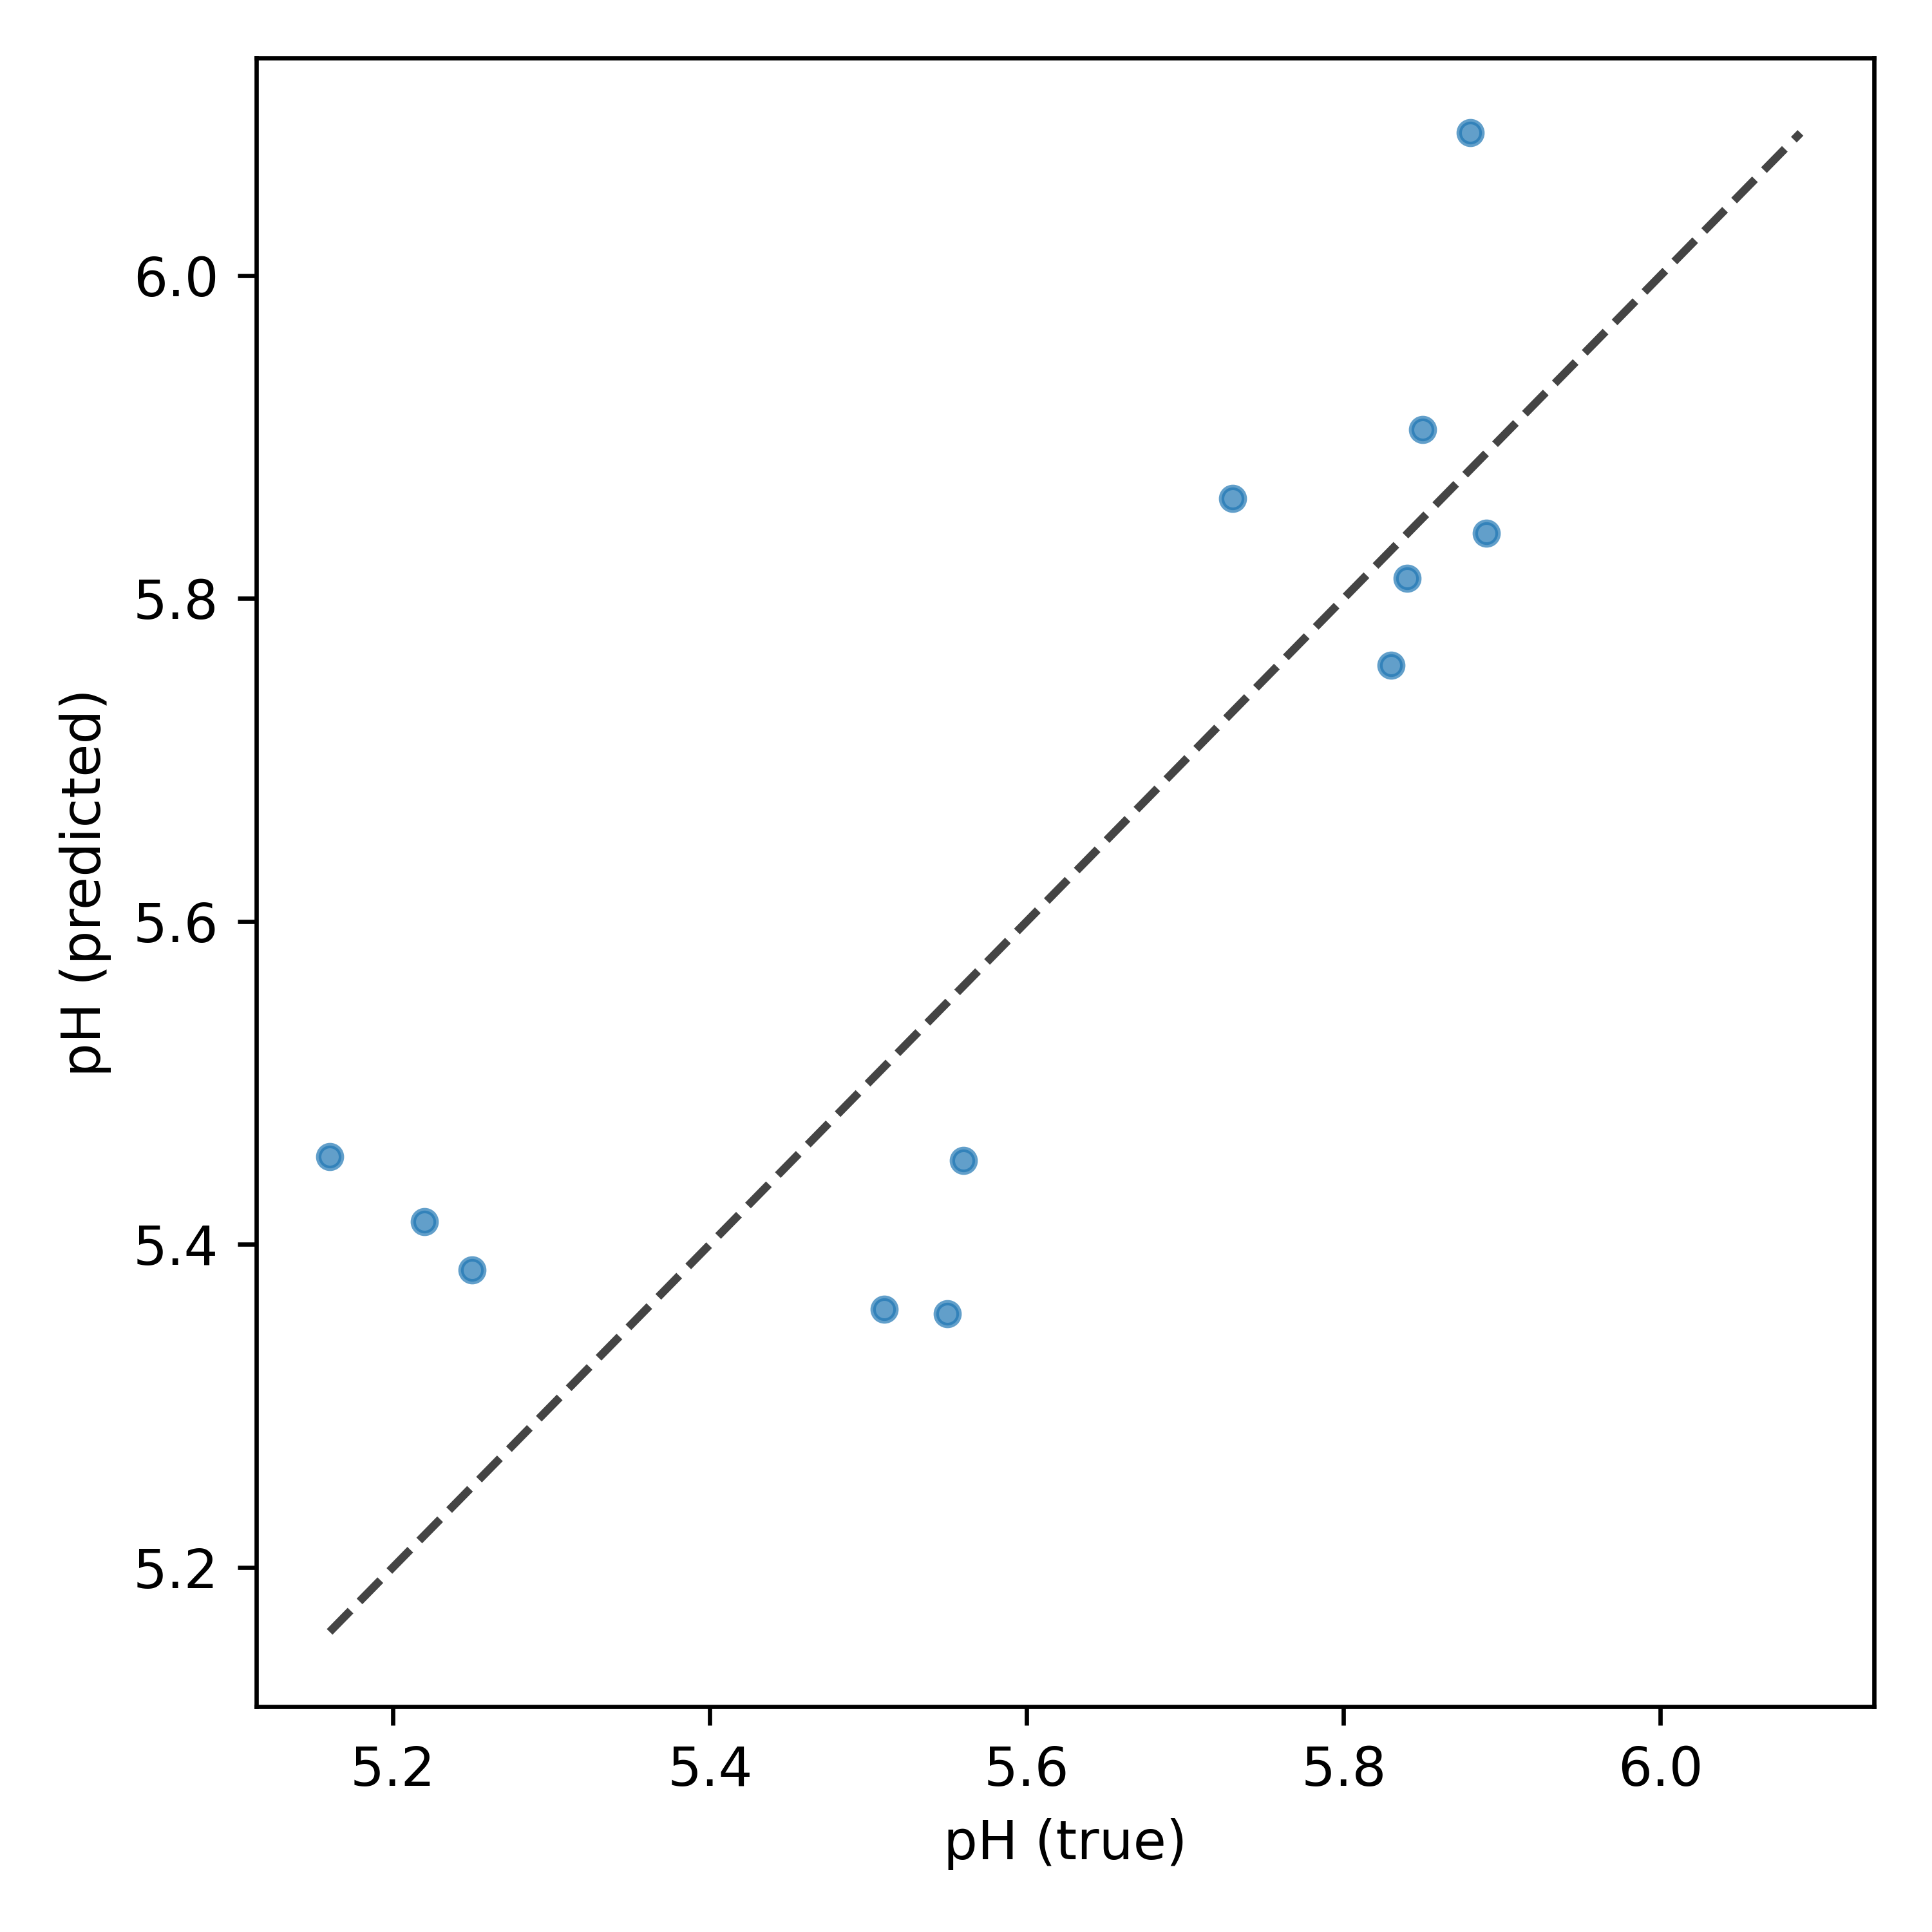
\includegraphics[width=\linewidth]{pred_vs_real_pH_multi.png}
\par\vspace{1mm}{\footnotesize (a) pH\par}
\end{minipage}\hspace{6mm}
\begin{minipage}{0.21\textwidth}
\centering
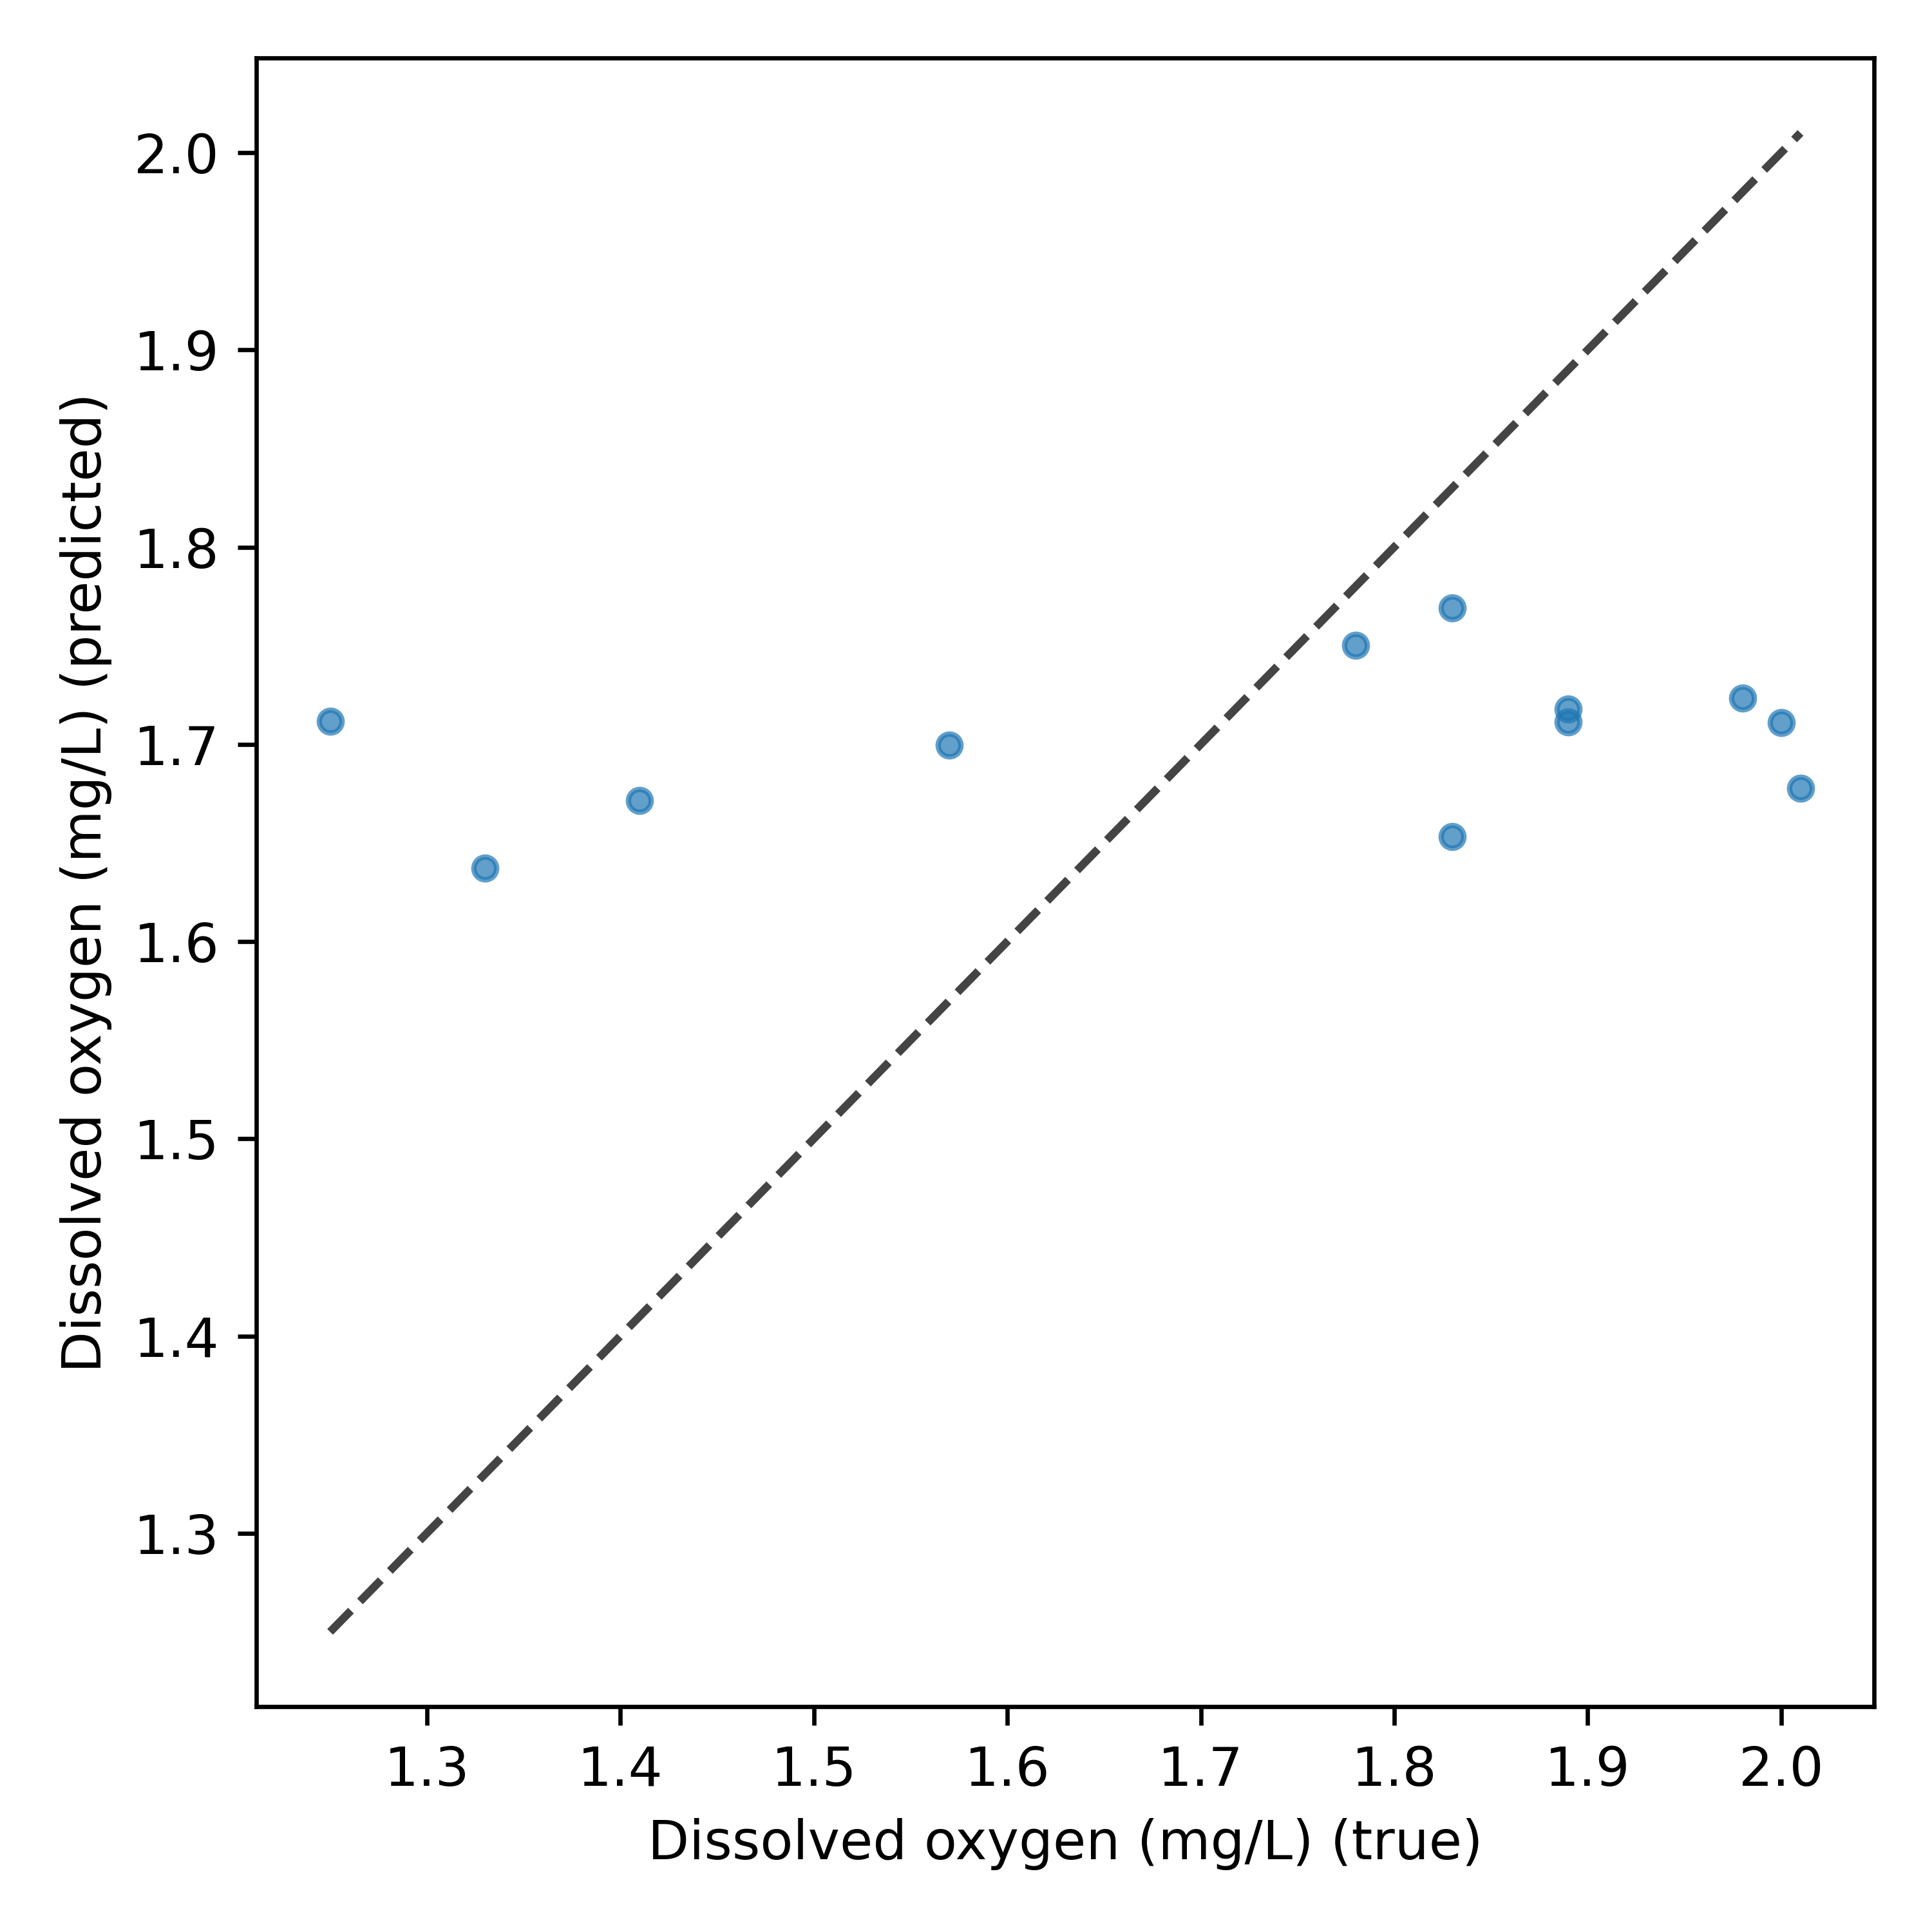
\includegraphics[width=\linewidth]{pred_vs_real_OD_multi.png}
\par\vspace{1mm}{\footnotesize (b) OD\par}
\end{minipage}\hspace{6mm}
\begin{minipage}{0.21\textwidth}
\centering
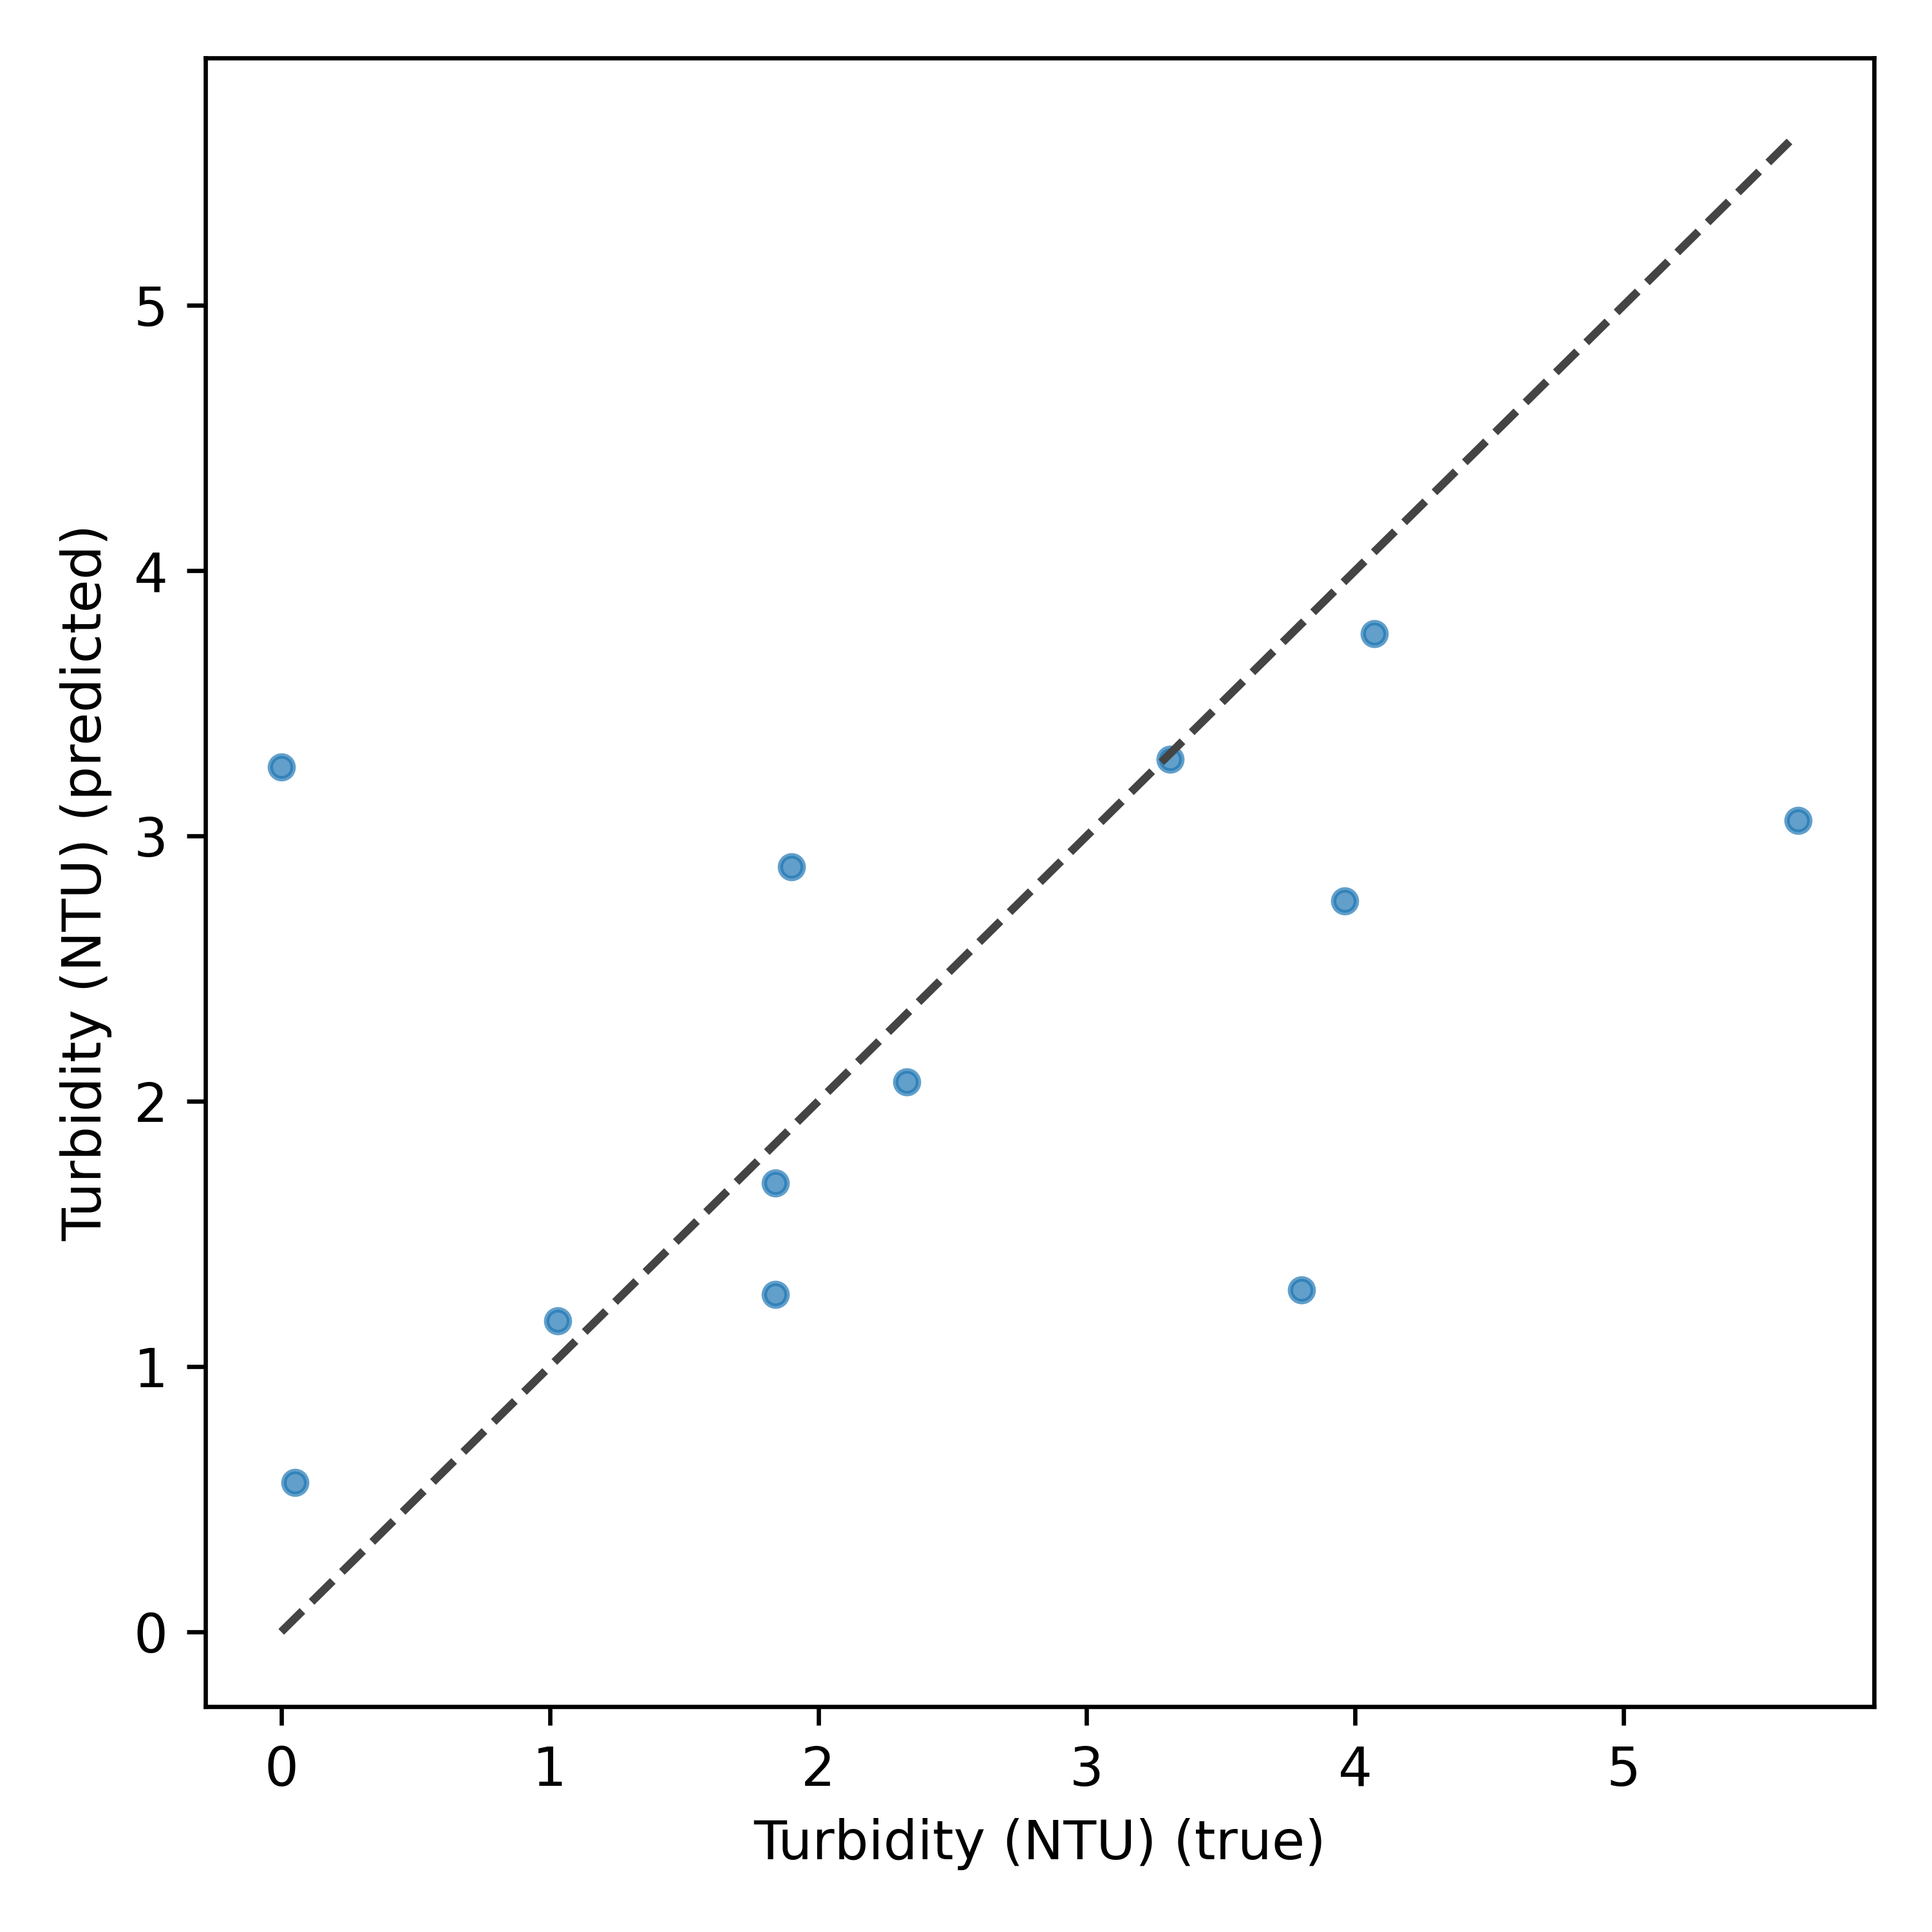
\includegraphics[width=\linewidth]{pred_vs_real_TURB_multi.png}
\par\vspace{1mm}{\footnotesize (c) TURB\par}
\end{minipage}
\caption{Valores preditos vs.\ reais na SNN multimodal para pH, oxigênio dissolvido e turbidez. \rev{(Figura ampliada para a largura total da página nesta revisão, para legibilidade dos eixos.)}}
\label{fig:pred_true_multi_sba}
\end{figure*}

\subsection{Resultados Espaciais e Índice de Poluição}
A interpolação IDW foi usada para converter predições pontuais em superfícies espaciais contínuas, melhorando a interpretação ambiental para além das métricas pontuais. Como mostra a Figura~\ref{fig:idw_combined_sba}, os mapas resultantes evidenciam comportamento espacial não uniforme de pH, oxigênio dissolvido e turbidez, e indicam microzonas candidatas para inspeção de campo priorizada.

\begin{figure*}[!t]
\centering
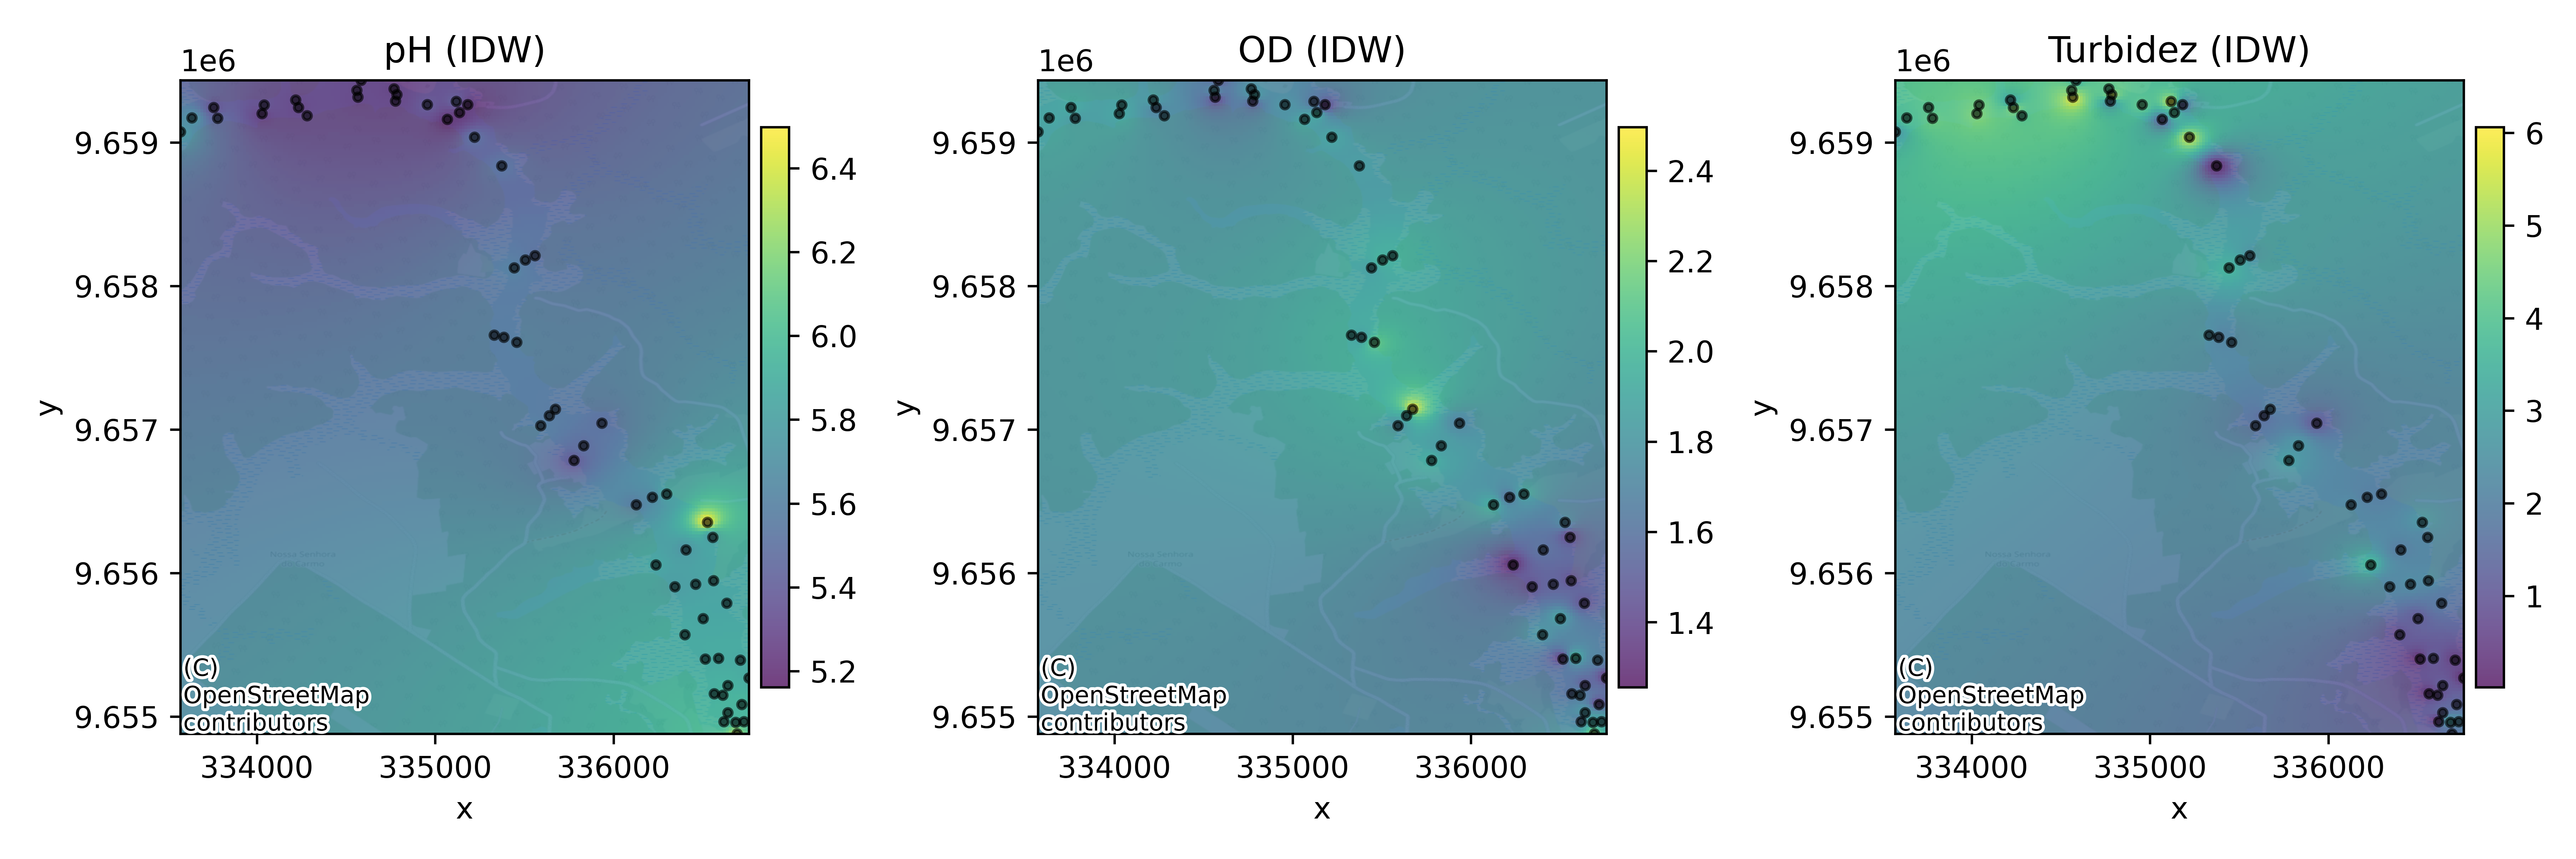
\includegraphics[width=0.70\textwidth]{idw_combined.png}
\caption{Superfícies interpoladas por IDW para pH, oxigênio dissolvido e turbidez a partir dos pontos amostrados. \rev{(Figura ampliada para a largura total da página nesta revisão, para legibilidade dos eixos.)}}
\label{fig:idw_combined_sba}
\end{figure*}

Para apoiar a triagem operacional, um índice composto de poluição foi calculado a partir das predições multimodais e normalizado para \mbox{$[0,1]$}, em que valores mais altos indicam pior condição relativa dentro do conjunto analisado. Como ilustra a Figura~\ref{fig:pollution_sba}, a representação em nível de ponto e sua estimativa espacial por IDW sobre o mapa-base OSM fornecem uma ferramenta visual direta para a identificação de áreas críticas.

\begin{figure*}[!t]
\centering
\begin{minipage}[t]{0.28\textwidth}
\centering
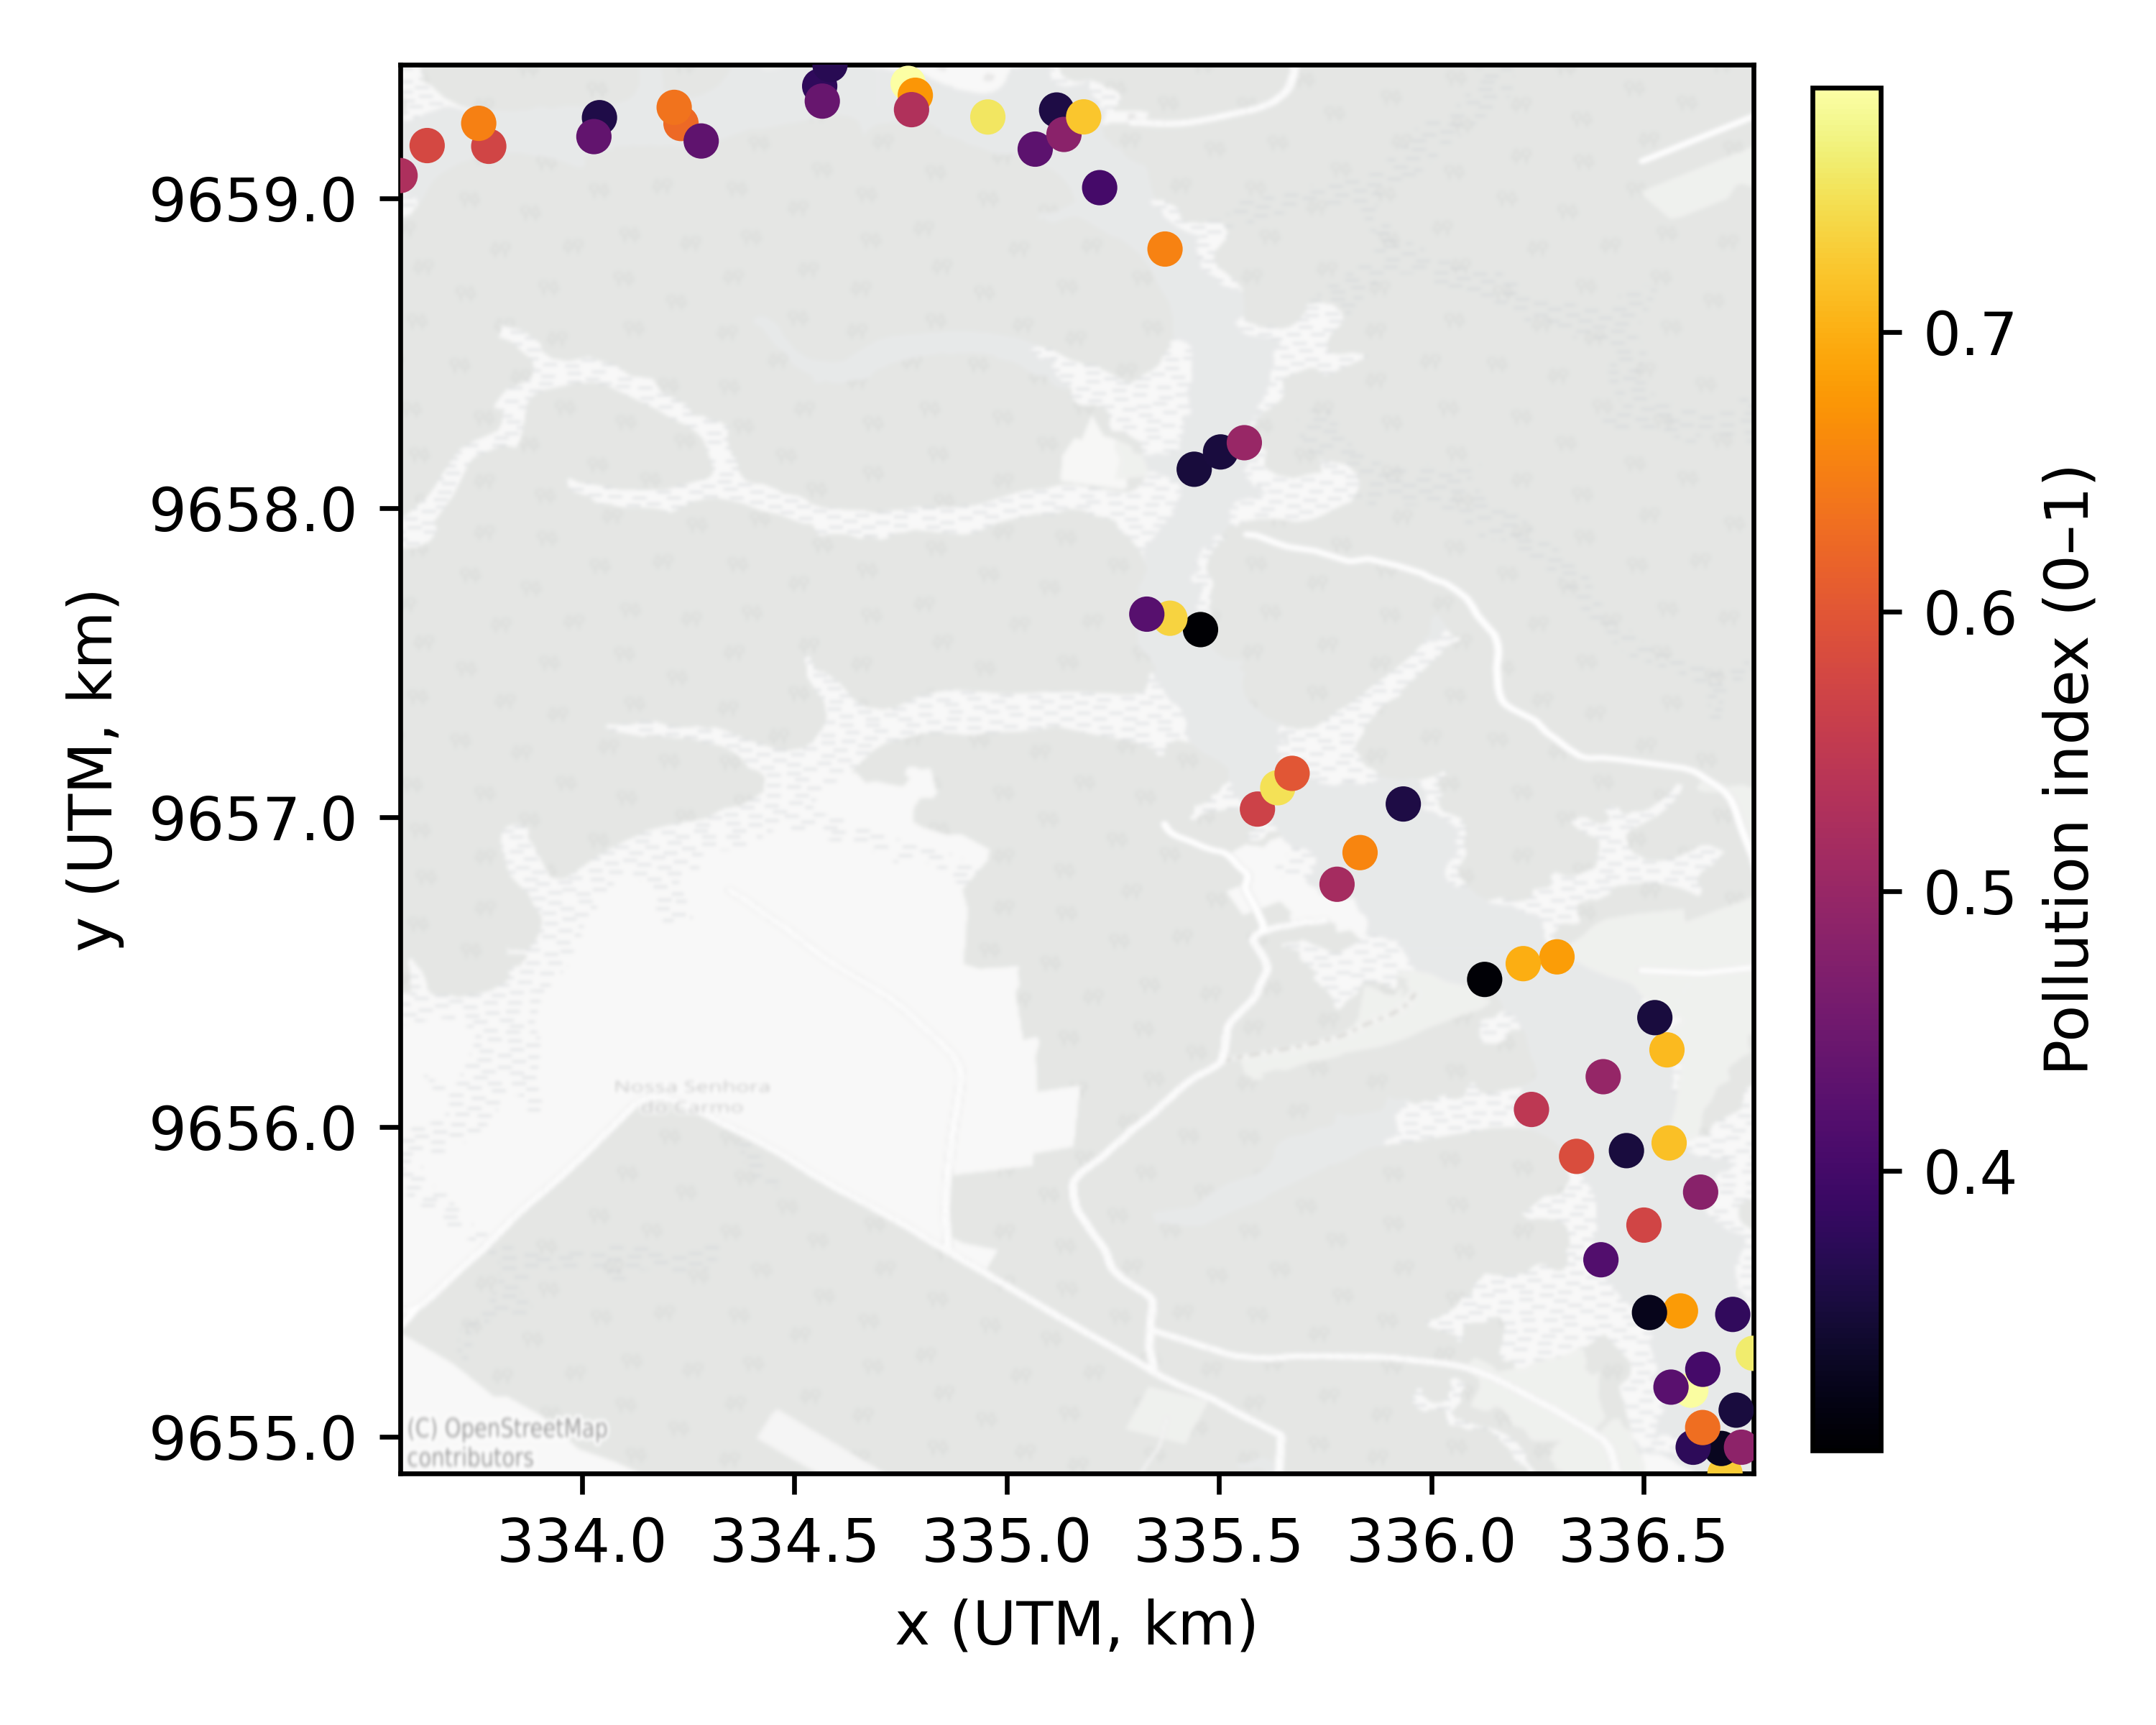
\includegraphics[width=\linewidth]{pollution_scatter.png}
\par\vspace{1mm}{\footnotesize (a) Índice de poluição nos pontos amostrados.\par}
\end{minipage}\hspace{8mm}
\begin{minipage}[t]{0.28\textwidth}
\centering
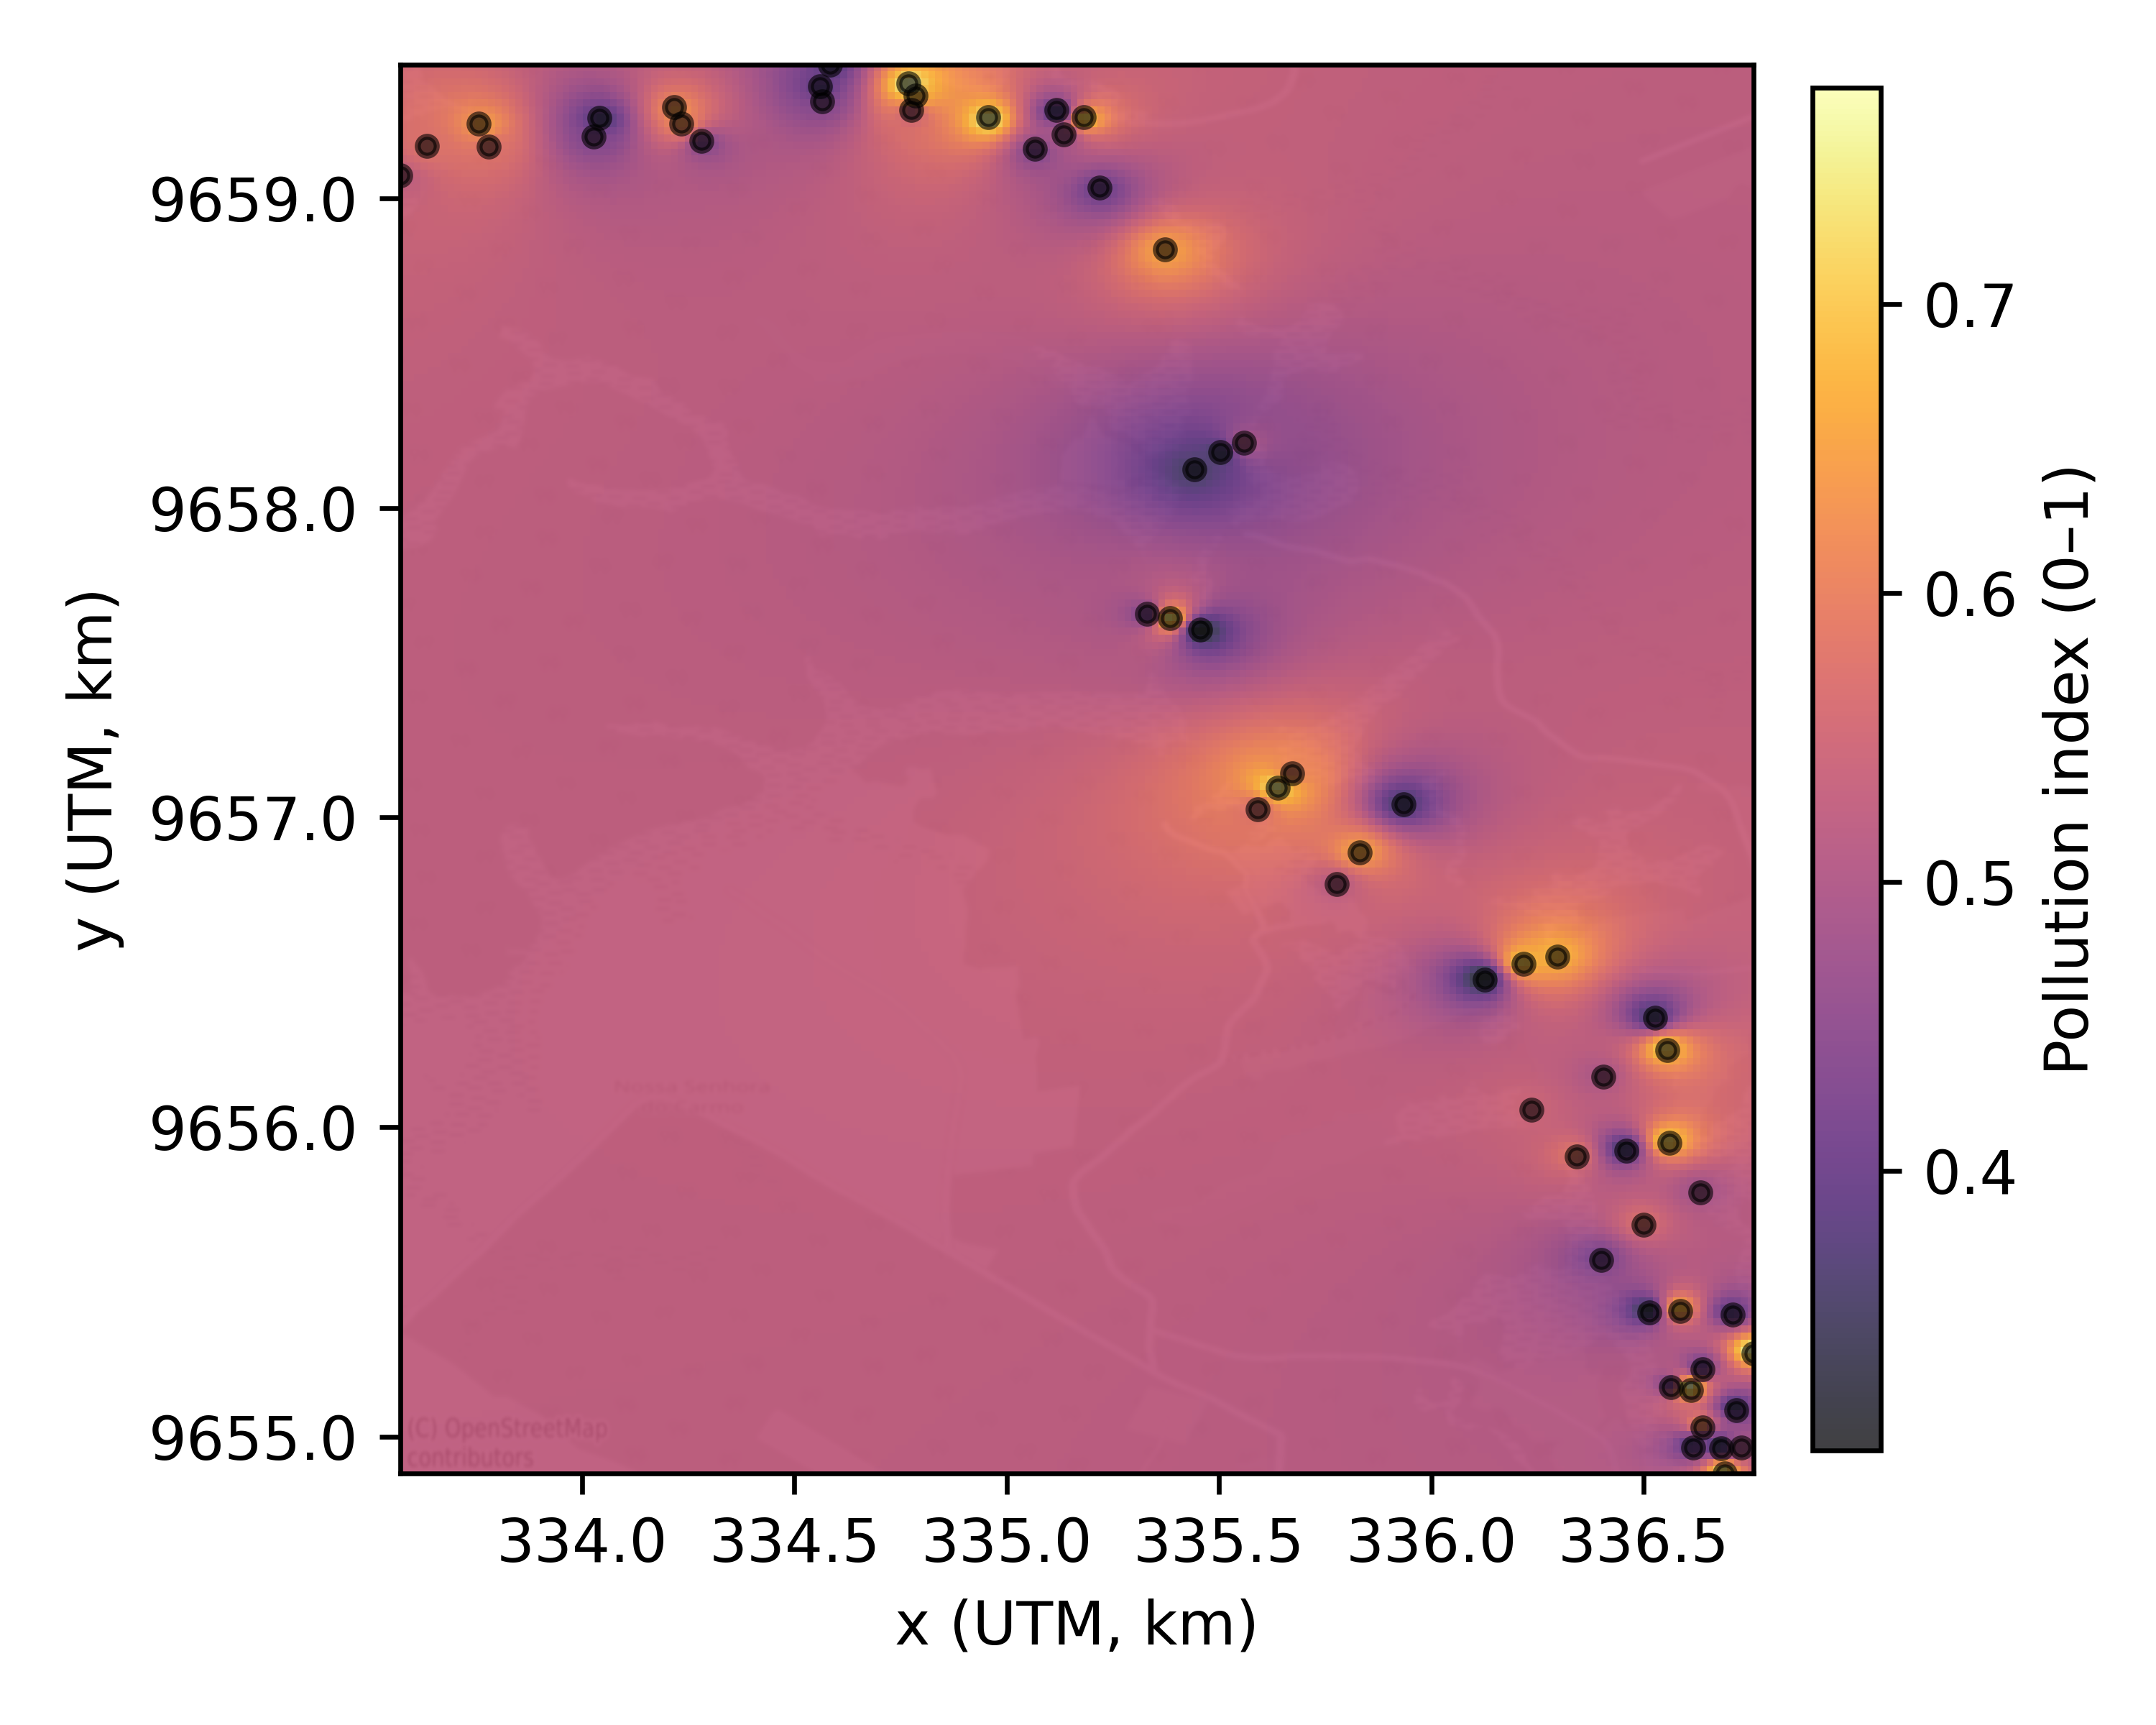
\includegraphics[width=\linewidth]{pollution_idw.png}
\par\vspace{1mm}{\footnotesize (b) Superfície IDW do índice.\par}
\end{minipage}
\caption{Estimativa espacial do índice composto de poluição a partir das predições multimodais (escala normalizada $[0, 1]$) sobre mapa-base OpenStreetMap (UTM 21S). \rev{(Figura ampliada para a largura total da página nesta revisão, para legibilidade dos eixos.)}}
\label{fig:pollution_sba}
\end{figure*}

\subsection{Consumo de Energia e Latência}
A Tabela~\ref{tab:energy_latency} reporta a energia incremental por inferência e a vazão nas plataformas de implantação. O ESP32 é viável para cenários autônomos de baixa taxa, mas apresenta maior energia por inferência devido à vazão limitada. Raspberry Pi e dispositivos Android fornecem mJ/inf muito menores em configurações de alta vazão.

\begin{table}[!htbp]
\caption{Latência/vazão e energia incremental nas plataformas.}
\label{tab:energy_latency}
\centering
\footnotesize
\setlength{\tabcolsep}{3pt}
\begin{tabular}{lccc}
\toprule
Plataforma & Vazão (amostras/s) & $\Delta P$ (W) & $E$ (mJ/inf) \\
\midrule
ESP32 (MicroPy) & 5.0 & 0.056 & 11.204 \\
Raspberry Pi 4B & 4670.50 & 0.239 & 0.0512 \\
Android A & 12337.40 & 0.128 & 0.0104 \\
Android B & 30905.08 & 0.468 & 0.0151 \\
Android C & 16121.71 & 0.046 & 0.00285 \\
\bottomrule
\end{tabular}
\end{table}

A Figura~\ref{fig:energy_bar_lnncs} compara a energia incremental por inferência em escala logarítmica: o ESP32 tem o maior custo por predição, principalmente devido à baixa vazão, enquanto Raspberry Pi e dispositivos Android operam em uma faixa de mJ/inf muito menor; maior vazão nem sempre implica menor energia por inferência, de modo que a seleção de plataforma deve considerar conjuntamente velocidade e potência incremental.

\begin{figure}[!htbp]
\centering
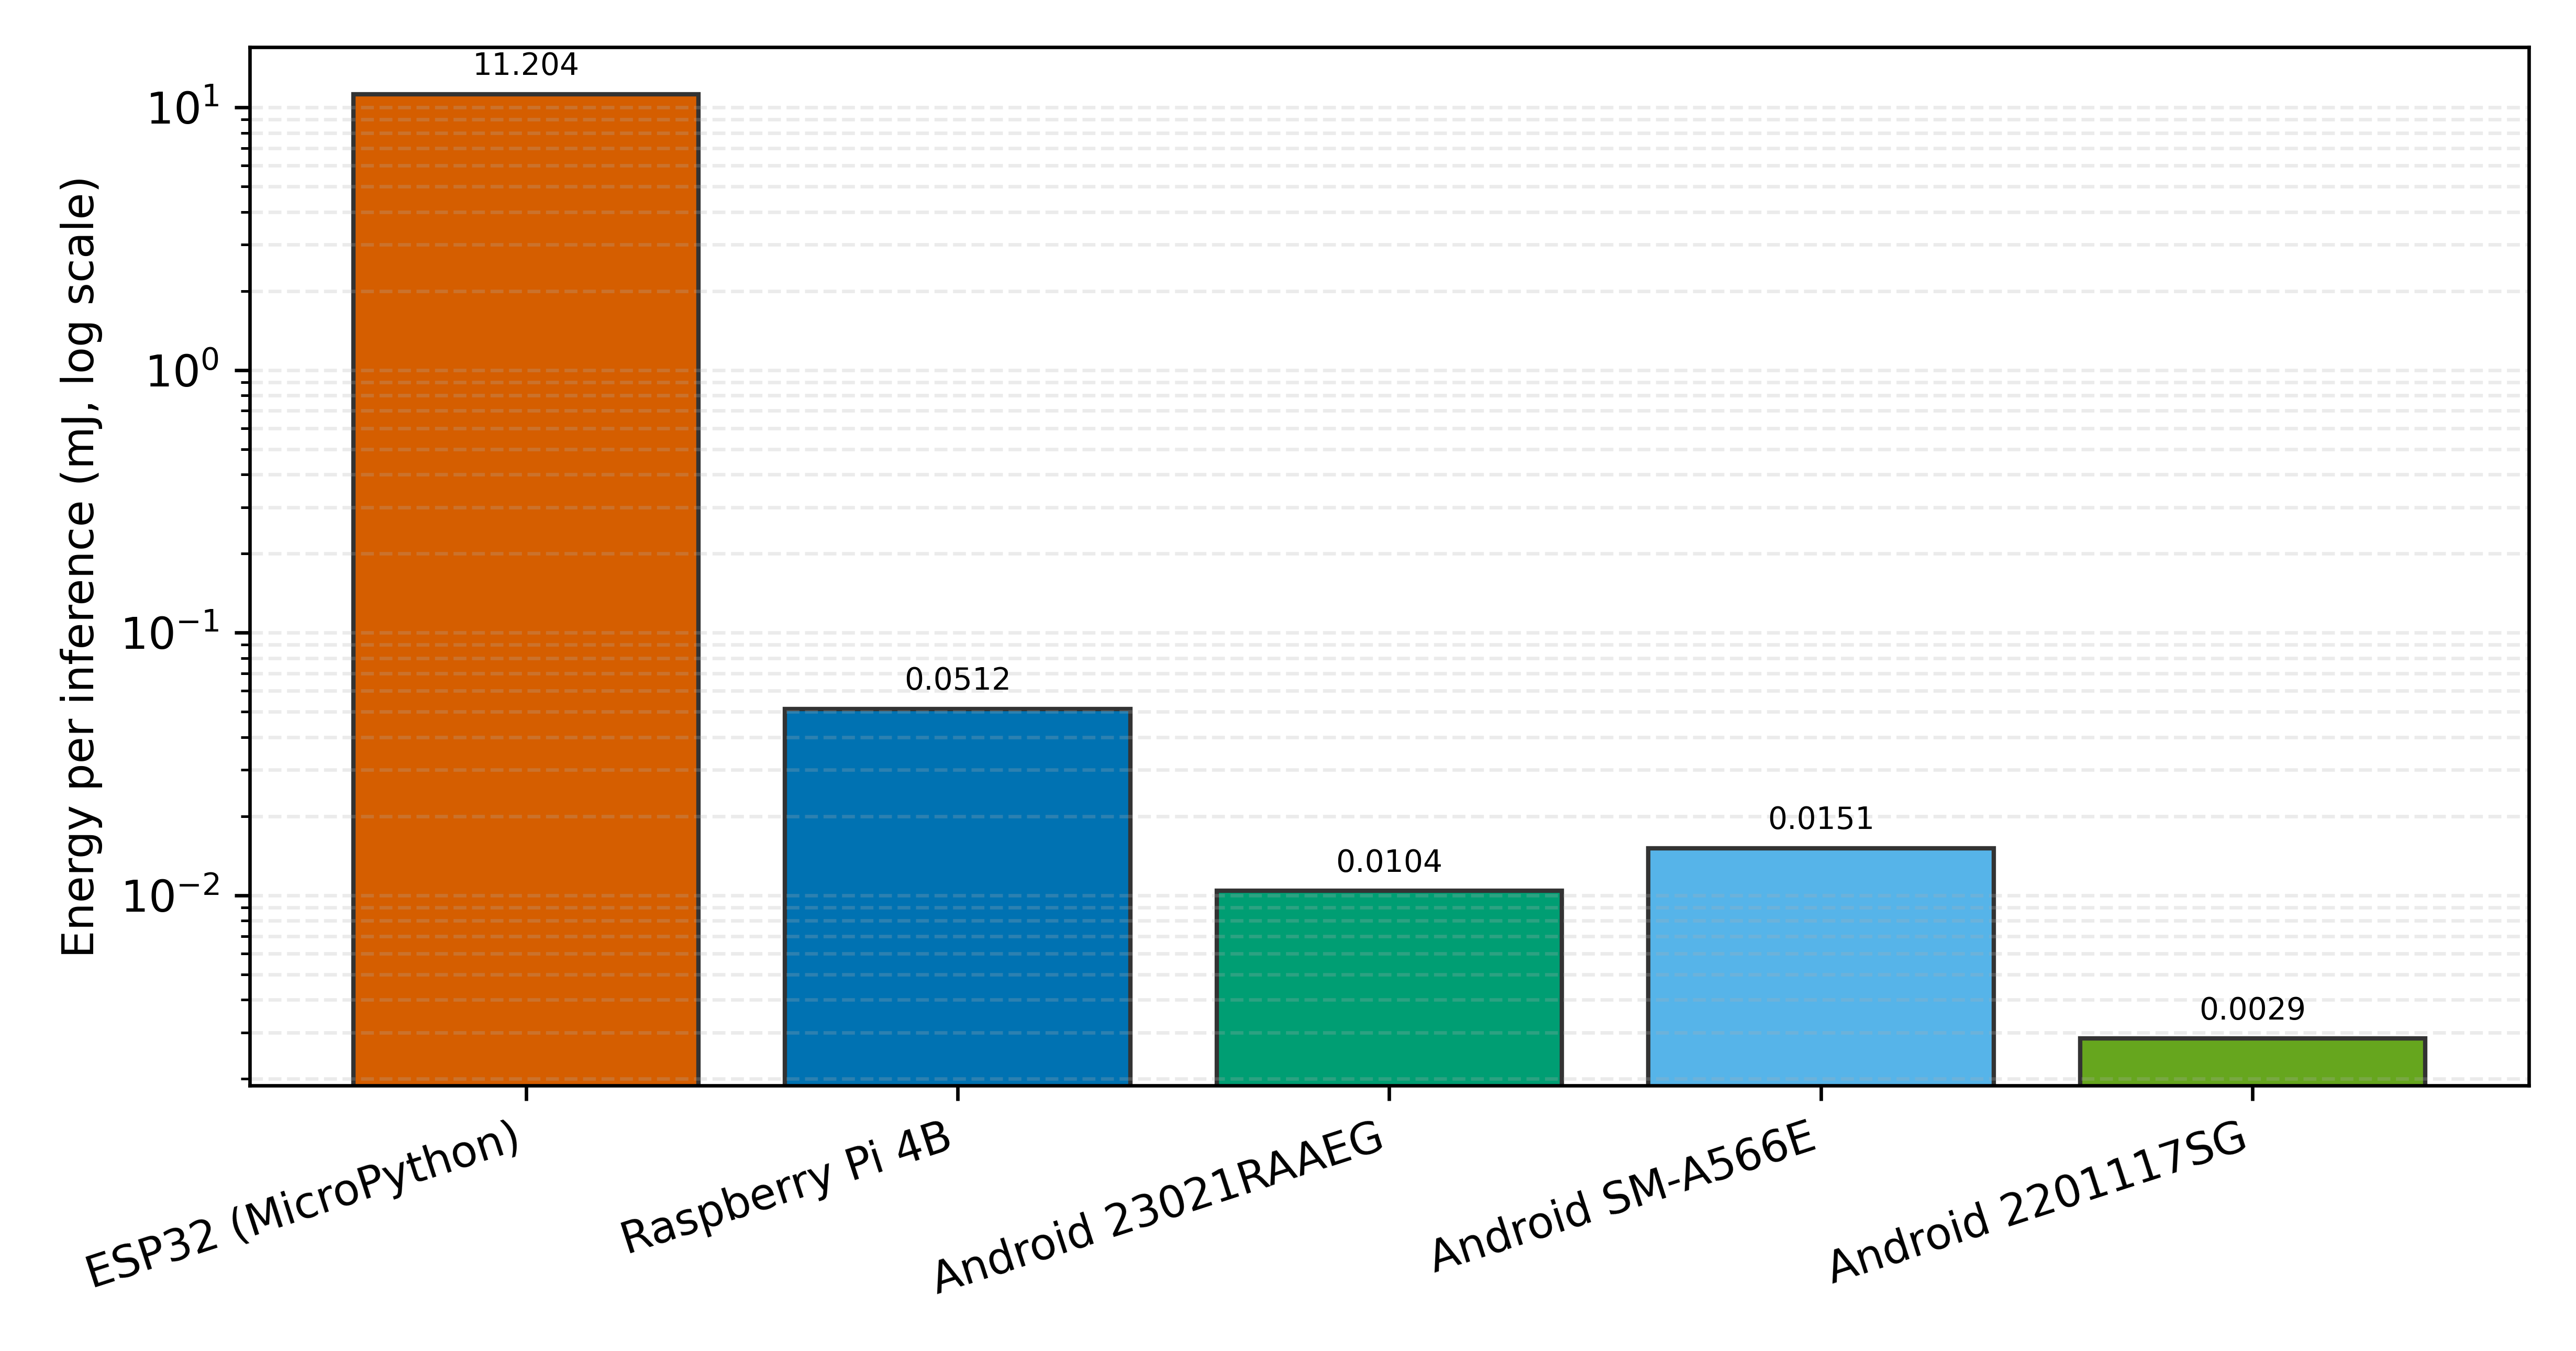
\includegraphics[width=\linewidth]{energy_platforms_bar.png}
\caption{Comparação da energia por inferência (escala logarítmica). \rev{(Figura ampliada nesta revisão para legibilidade dos eixos.)}}
\label{fig:energy_bar_lnncs}
\end{figure}

A Figura~\ref{fig:snn_platform_radar_sba} resume o envelope de implantação multicritério (vazão, latência inversa, energia inversa e referência preditiva) e mostra que nenhuma plataforma domina todos os objetivos: dispositivos Android e Raspberry Pi favorecem amostragem mais densa e fluxos interativos, enquanto o ESP32 permanece relevante para operação esparsa, autônoma e totalmente offline. A figura deve ser lida como um mapa de implantação, e não como um ranqueamento universal.

\begin{figure}[!t]
\centering
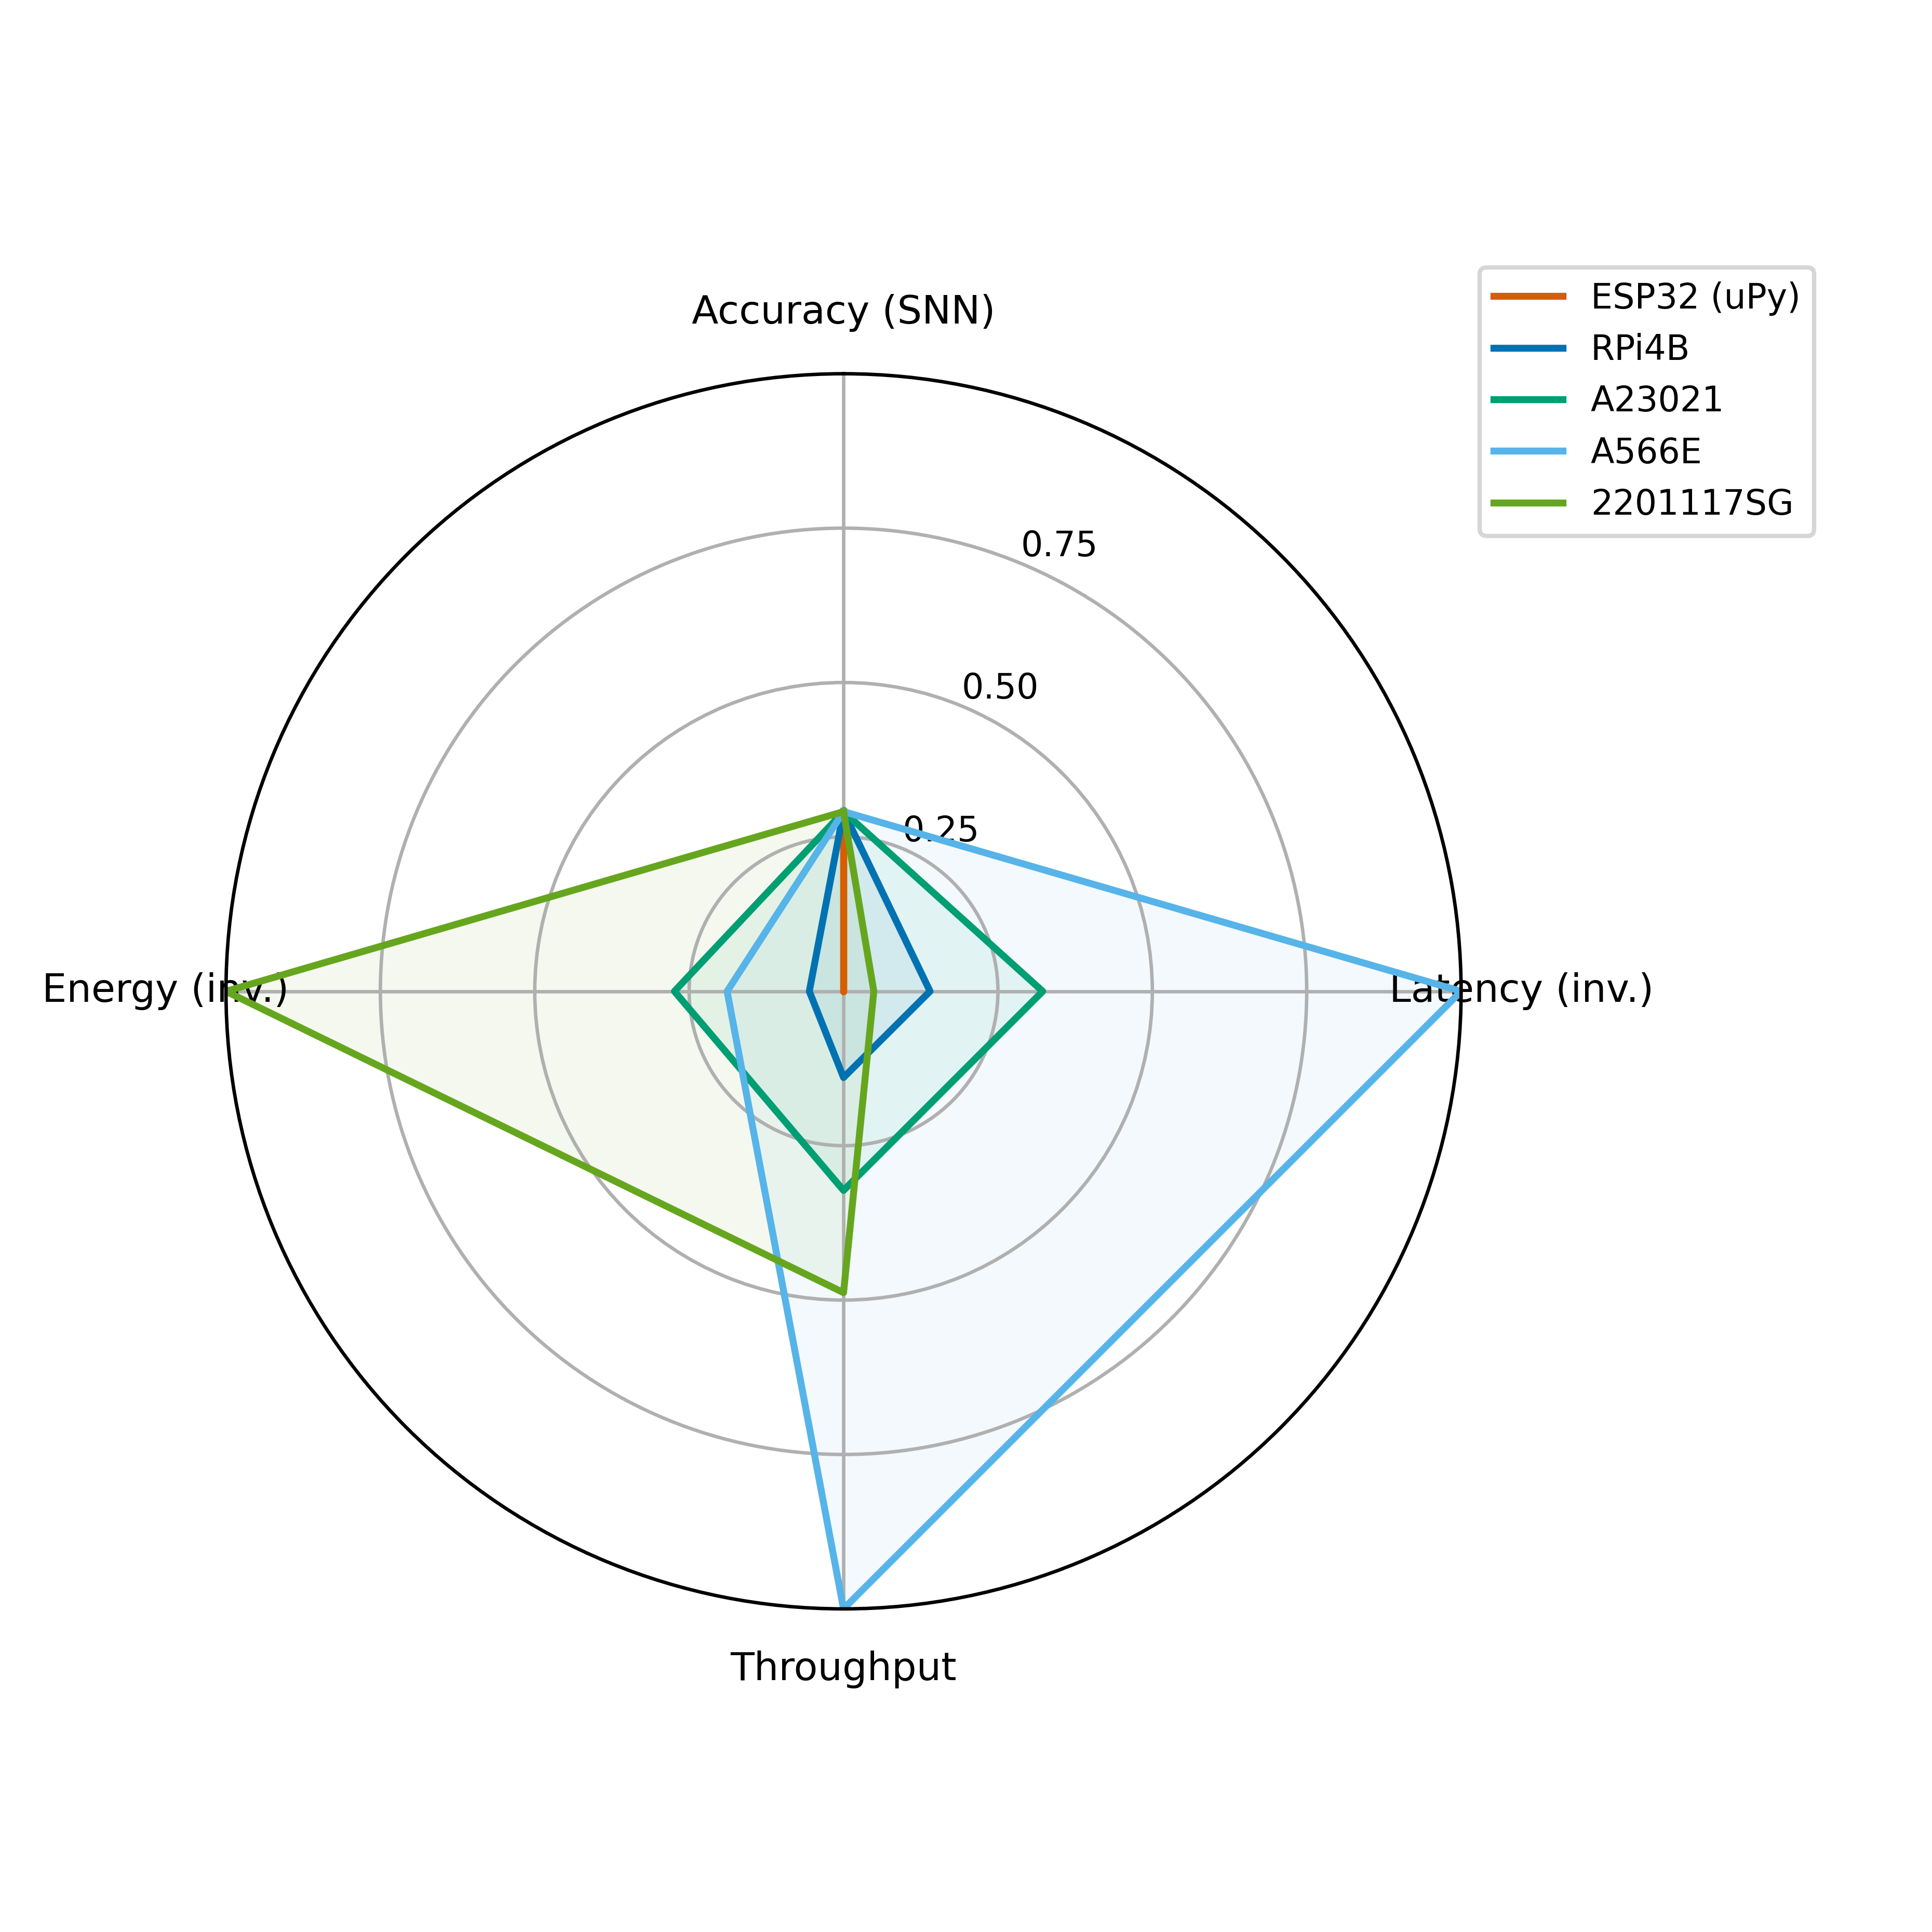
\includegraphics[width=0.52\linewidth]{snn_platform_radar.png}
\caption{Comparação da implantação da SNN entre plataformas usando critérios normalizados (vazão, latência inversa, energia inversa e referência preditiva). \rev{(Figura ampliada nesta revisão para legibilidade dos eixos.)}}
\label{fig:snn_platform_radar_sba}
\end{figure}
